%%%%%%%%%%%%%%%%%%%%%%%%%%%%%%%%%%%%%%%%%
% Simple Sectioned Essay Template
% LaTeX Template
%
% This template has been downloaded from:
% http://www.latextemplates.com
%
% Note:
% The \lipsum[#] commands throughout this template generate dummy text
% to fill the template out. These commands should all be removed when 
% writing essay content.
%
%%%%%%%%%%%%%%%%%%%%%%%%%%%%%%%%%%%%%%%%%

%----------------------------------------------------------------------------------------
%	PACKAGES AND OTHER DOCUMENT CONFIGURATIONS
%----------------------------------------------------------------------------------------

\documentclass[12pt]{report} % Default font size is 12pt

\usepackage[utf8]{inputenc}

\usepackage[a4paper]{geometry} % Required to change the page size to A4
% Set the page size to be A4 as opposed to the default US Letter

\usepackage{float} % Allows putting an [H] in \begin{figure} to specify the exact location of the figure
\usepackage{wrapfig} % Allows in-line images such as the example fish picture

\usepackage{lipsum} % Used for inserting dummy 'Lorem ipsum' text into the template

\usepackage{amsmath}
\usepackage{amsthm}
\usepackage{amssymb}

\usepackage[nottoc]{tocbibind}

\usepackage{makeidx}
\makeindex

\linespread{1.2} % Line spacing

%\setlength\parindent{0pt} % Uncomment to remove all indentation from paragraphs

\usepackage{graphicx} % Required for including pictures

\graphicspath{{../figures/}} % Specifies the directory where pictures are stored

\usepackage{hyperref}
\hypersetup{
    colorlinks,
    citecolor=black,
    filecolor=black,
    linkcolor=black,
    urlcolor=black
}

\usepackage{microtype}
\usepackage{siunitx}
\usepackage{cleveref}
\usepackage{booktabs}

\begin{document}

%----------------------------------------------------------------------------------------
%	TITLE PAGE
%----------------------------------------------------------------------------------------

\begin{titlepage}

\newcommand{\HRule}{\rule{\linewidth}{0.5mm}} % Defines a new command for the horizontal lines, change thickness here

\center % Center everything on the page

\textsc{\Large The University of New South Wales}\\[0.2cm]
\textsc{\large School of Computer Science and Engineering}\\[1.5cm] % Name of your university/college

\textsc{\large Thesis Report - Part A}\\[0.5cm] % Major heading such as course name
\textsc{BSc Computer Science (Honours)}\\[0.5cm] % Minor heading such as course title

\HRule \\[0.4cm]
{ \LARGE \bfseries The Chromatic Derivatives and its Applications }\\[0.4cm] % Title of your document
\HRule \\[1.5cm]

\begin{minipage}[t]{0.4\textwidth}
\begin{flushleft} \large
\emph{Author:}\\
Louis \textsc{Tiao} % Your name
\end{flushleft}
\end{minipage}
~
\begin{minipage}[t]{0.5\textwidth}
\begin{flushright} \large
\emph{Supervisor:} \\
Dr. Aleksandar \textsc{Ignjatovic} % Supervisor's Name
\\[0.5cm]
\emph{Assessor:} \\
Dr. Alan \textsc{Blair} % Assessor's Name
\end{flushright}
\end{minipage}\\[4cm]

{\large \today}\\[3cm] % Date, change the \today to a set date if you want to be precise

%\includegraphics{Logo}\\[1cm] % Include a department/university logo - this will require the graphicx package

\vfill % Fill the rest of the page with whitespace

\end{titlepage}

%----------------------------------------------------------------------------------------
%	TABLE OF CONTENTS
%----------------------------------------------------------------------------------------

\tableofcontents % Include a table of contents

\newpage % Begins the essay on a new page instead of on the same page as the table of contents 

%----------------------------------------------------------------------------------------
%	INTRODUCTION
%----------------------------------------------------------------------------------------

\chapter{Introduction} % Major section
Example citation \cite{Ignjatovic2009}.

%------------------------------------------------

\section{Subsection 1} % Sub-section

\begin{itemize}
	\item Let $f(t)$ be a signal in the time domain with period $2T$. Its 
		\textit{Fourier series} \index{Fourier series} expansion is given by

		\begin{align}
			f(t)	&= \sum_{n=-\infty}^{\infty} c_n e^{i \frac{\pi n}{T} t} \\
			c_n		&= \frac{1}{2T} \int_{-T}^{T} f(t) e^{-i \frac{\pi n}{T} t} dt
		\end{align}
	\item \textbf{Global}, approximates local behaviour poorly
	\item Indispensable to digital signal processing (DSP)
	% TODO: Insert complex exponential identities (?)
\end{itemize}

\lipsum[1] % Dummy text

%------------------------------------------------

\section{Subsection 2} % Sub-section

\lipsum[2] % Dummy text

%------------------------------------------------
\chapter{Background}

\section{Mathem}

\section{Digital signal processing}

\section{Computer vision and Image processing}

\subsubsection{Subsubsection 1} % Sub-sub-section

\lipsum[3] % Dummy text

\begin{figure}[H] % Example image
\center{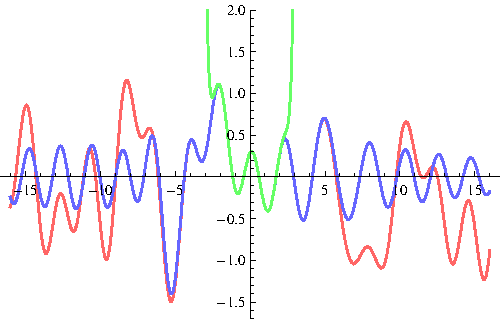
\includegraphics[width=0.5\linewidth]{approx}}
\caption{Example image.}
\label{fig:speciation}
\end{figure}

%------------------------------------------------

\subsubsection{Subsubsection 2} % Sub-sub-section

\lipsum[4] % Dummy text

%----------------------------------------------------------------------------------------
%	MAJOR SECTION 1
%----------------------------------------------------------------------------------------

\chapter{Content Section} % Major section

\lipsum[5] % Dummy text

%------------------------------------------------

\section{Subsection 1} % Sub-section

\subsubsection{Subsubsection 1} % Sub-sub-section

\lipsum[6] % Dummy text

%------------------------------------------------

\subsubsection{Subsubsection 2} % Sub-sub-section

\lipsum[6] % Dummy text
\begin{wrapfigure}{l}{0.4\textwidth} % Inline image example
  \begin{center}
    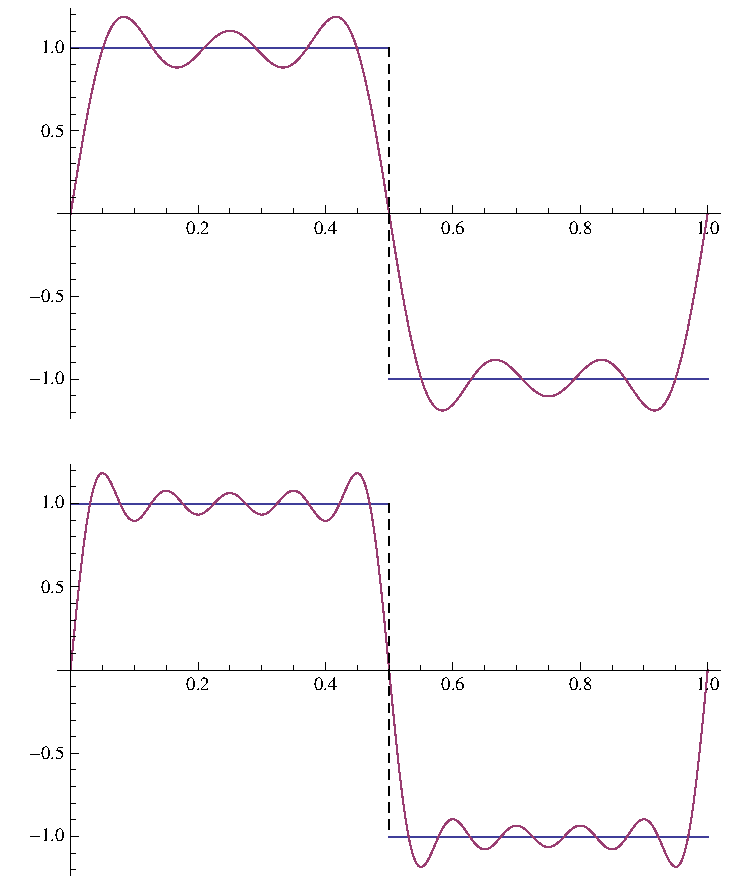
\includegraphics[width=0.38\textwidth]{fourier}
  \end{center}
  \caption{Fish}
\end{wrapfigure}
\lipsum[7-8] % Dummy text

%------------------------------------------------

\subsubsection{Subsubsection 3} % Sub-sub-section

\begin{description} % Numbered list example

\item[First] \hfill \\
\lipsum[9] % Dummy text

\item[Second] \hfill \\
\lipsum[10] % Dummy text

\item[Third] \hfill \\
\lipsum[11] % Dummy text

\end{description} 

%----------------------------------------------------------------------------------------
%	MAJOR SECTION X - TEMPLATE - UNCOMMENT AND FILL IN
%----------------------------------------------------------------------------------------

%\chapter{Content Section}

%\section{Subsection 1} % Sub-section

% Content

%------------------------------------------------

%\section{Subsection 2} % Sub-section

% Content

%----------------------------------------------------------------------------------------
%	CONCLUSION
%----------------------------------------------------------------------------------------

\chapter{Conclusion} % Major section

\lipsum[12-13]

%----------------------------------------------------------------------------------------
%	BIBLIOGRAPHY
%----------------------------------------------------------------------------------------

\bibliographystyle{plain}
\bibliography{../bibliography}

%----------------------------------------------------------------------------------------
%	APPENDIX
%----------------------------------------------------------------------------------------

\appendix

\chapter{Code}

%----------------------------------------------------------------------------------------
%	INDEX
%----------------------------------------------------------------------------------------

\printindex

%----------------------------------------------------------------------------------------

\end{document}